%!Mode:: "TeX:UTF-8"
 
\section{外设}


\begin{figure}[ht]
	\begin{center}
		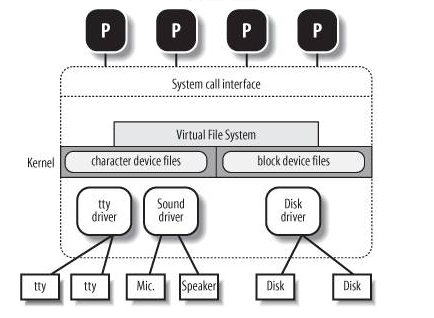
\includegraphics[keepaspectratio,width=0.5\paperwidth]{Pictures/Kernel/LinuxDriverInf.png}
	\caption{Linux外设接口模型}
	\label{fig:LinuxDriverInf}
	\end{center}
\end{figure}

\begin{figure}[ht]
	\begin{center}
		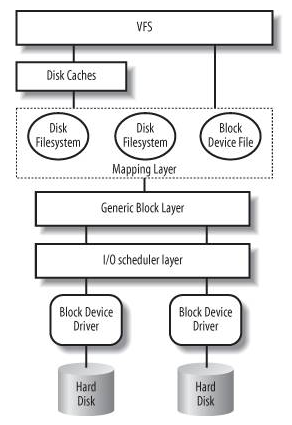
\includegraphics[keepaspectratio,width=0.4\paperwidth]{Pictures/Kernel/kernelComponentForBlockDeviceOp.png}
	\caption{与块设备操作相关的内核组件}
	\label{fig:kernelComponentForBlockDeviceOp}
	\end{center}
\end{figure}

在对块设备进行I/O操作时,图 \ref{fig:kernelComponentForBlockDeviceOp}中的映射层将”文件偏移量,读写长度“数值对映射为若干组连续的磁盘逻辑块,必要时借助文件系统(读取inode)。
通用块层对每组连续的块发起BIO操作。
内核中用inode结构表示索引节点,可以是文件,也可以是目录。inode(可理解为ext2 inode)对应于物理磁盘上的具体对象。


\begin{figure}[ht]
	\begin{center}
		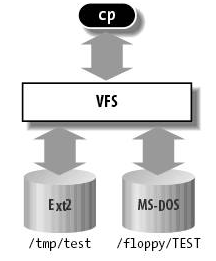
\includegraphics[keepaspectratio,width=0.15\paperwidth]{Pictures/Kernel/VirtualFileSystem.png}
	\caption{VFS在copy操作中的作用}
	\label{fig:VirtualFileSystem}
	\end{center}
\end{figure}


\begin{figure}[ht]
	\begin{center}
		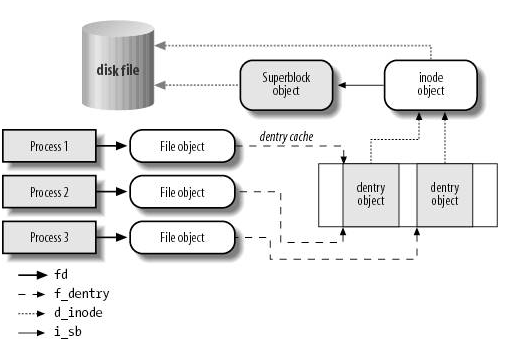
\includegraphics[keepaspectratio,width=0.4\paperwidth]{Pictures/Kernel/LinuxProcessAndVFS.png}
	\caption{进程与VFS的交互}
	\label{fig:LinuxProcessAndVFS}
	\end{center}
\end{figure}

\begin{figure}[ht]
	\begin{center}
		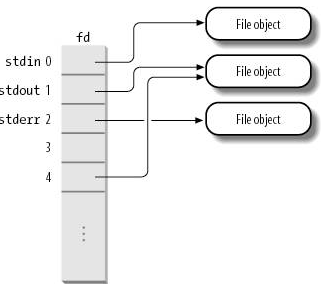
\includegraphics[keepaspectratio,width=0.3\paperwidth]{Pictures/Kernel/LinuxFdArrayInFileStruct.png}
	\caption{file\_struct中的fd数组}
	\label{fig:LinuxFdArrayInFileStruct}
	\end{center}
\end{figure}


\begin{figure}[ht]
	\begin{center}
		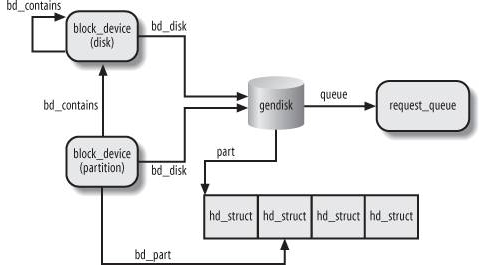
\includegraphics[keepaspectratio,width=0.6\paperwidth]{Pictures/Kernel/BlockDeviceDescriptors.png}
	\caption{块设备描述符}
	\label{fig:BlockDeviceDescriptors}
	\end{center}
\end{figure}













\clearpage

